\clearpage
\subsection{Experimental Result of DEF Expansion on Mechanical Properties of Concrete}

% Bruetaud et al., 2008
In first test study, Bruetaud et al.\cite{Bruetaud} observed DEF-affected concrete in views of compressive strength. Figure \ref{Bruetaud Mix designs} summarizes the mix designs of these different concretes.

\begin{figure}[h!]
  \centering
  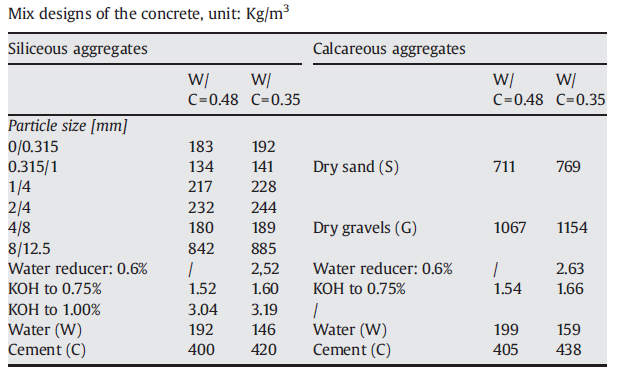
\includegraphics[width=0.8\linewidth]{Reference/Bruetaud1.png}
  \caption{Mix designs of the concrete, DEF cylinders[Bruetaud et al., 2008\cite{Bruetaud}]}
  \label{Bruetaud Mix designs}
\end{figure}

Each concrete sample was cast and cured in 3 cylindrical moulds whose dimensions are 11 cm (diameter) and 22 cm (height) to generate 3 identical concrete specimens. The moulds were covered so as to limit water exchange. The applied heat treatment followed a cycle divided into four different steps, as shown in Figure \ref{Bruetaud heat}. Some concrete samples were not heat treated but were conventionally cured at 20 $^\circ$C to be used as reference. After the heat treatment, samples were stored at 20 $^\circ$C in 100\% relative humidity until 28 days. Next, wetting and drying cycles were applied in accordance with LPC no. 59 pre-test method, to increase the kinetics of DEF reaction without changing its triggering conditions. Samples are subjected to 2 cycles, each one lasting 14 days. A cycle consists of 7 days of drying at 38 $^\circ$C and 30\% relative humidity followed by 7 days of immersion in tap water at 20 $^\circ$C. The volume of water with respect to the volume of the sample is kept under 1.5 to limit leaching effects. Once the cycles are finished, samples are stored into 3 individual hermetic boxes (to avoid carbonation) whose dimensions barely exceed those of the sample, to minimize the amount ofwater required for their immersion.[Bruetaud et al., 2008\cite{Bruetaud}]

\begin{figure}[h!]
  \centering
  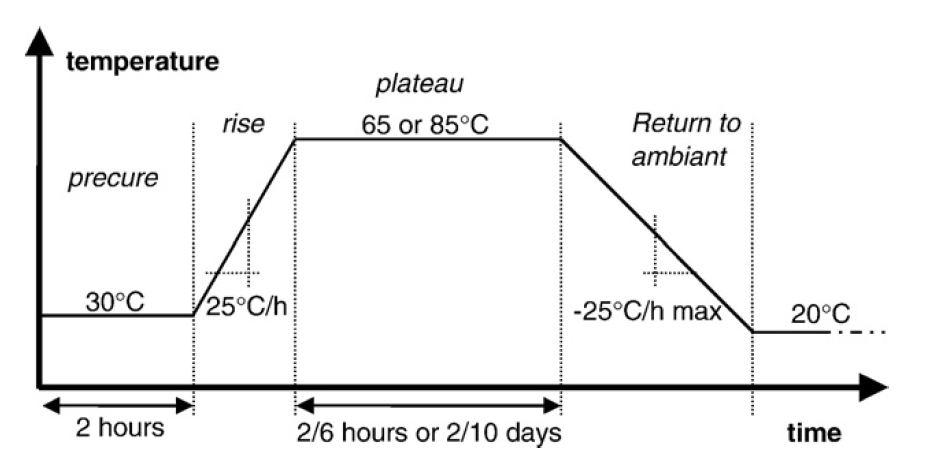
\includegraphics[width=0.8\linewidth]{Reference/Bruetaud2.png}
  \caption{Heat treatment phases of DEF cylinders[Bruetaud et al., 2008\cite{Bruetaud}]}
  \label{Bruetaud heat}
\end{figure}

During this last period, expansion measurements were performed with an extensometer whose resulting measurement dispersion on the basis of three concrete specimens is less than 0.002\%.

In the case of 0.48-Si concretes (“heating” experiments), a relationship can be obtained between the ultimate compressive strength (residual strength) and the final expansion achieved. Typically, the strength of unaffected 0.48-Si concrete specimens reaches about 40 MPa. The most damaged specimens of 0.48-Si concretes fall down to 15 MPa, which represents a very significant decrease.[Bruetaud et al., 2008]

In Figure \ref{Bruetaud CS}, the linear approximation would forecast a fall of strength on the order of 90\% for a 1.6\% expansion. This value, certainly exaggerated by the linear approximation, serves to verify that high expansion (over 1\%) leads to very low residual mechanical strength. The linear approximation proposed in Figure \ref{Bruetaud CS} seems to imply that a DEF-related expansion lower
than 0.20\% will not generate significant loss in compressive strength.[Bruetaud et al., 2008\cite{Bruetaud}]

\begin{figure}[h!]
  \centering
  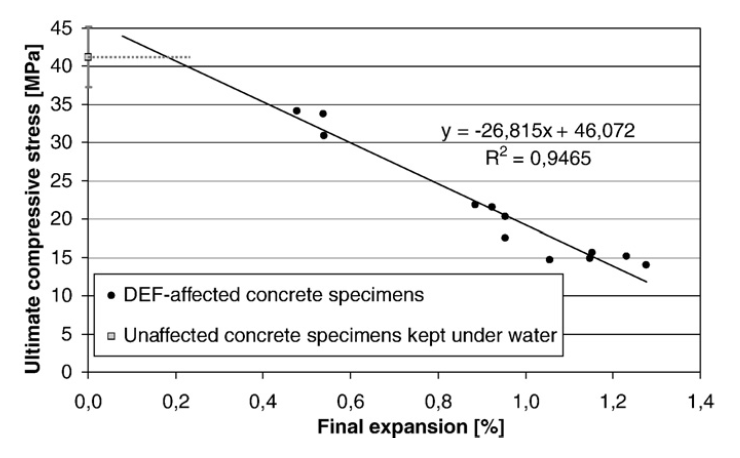
\includegraphics[width=0.8\linewidth]{Reference/Bruetaud3.png}
  \caption{Compressive stress versus final expansion for the concrete specimens of the
heating design of experiments[Bruetaud et al., 2008\cite{Bruetaud}]}
  \label{Bruetaud CS}
\end{figure}

\clearpage
% GIANNINI(2012)

Together with ASR expansion, Giannini\cite{GIANNINI} also carried out mechanical properties test on expanded specimens damaged by DEF expansion.

Similar two sets of 4 x 8 in. (100 x 200 mm) cylinders were produced for the purpose of further evaluating the mechanical properties of damaged concrete. Two types of aggregates, Jobe (F1) sand and Placitas (C10) gravel were used. A non-linear resonant frequency test method was also employed for selected test specimens. The cylinders are intended to represent a laboratory analog for core samples extracted from a field structure.

Here the experiment results for DEF expansion are presented. Figure \ref{Giannini, 2012 DEF} shows the compressive strength results for the Jobe (F1) andPlacitas (C10) cylinders, respectively. Each data represents the average of three cylinders. For the Jobe (F1) cylinders, decreases of 41\% were measured. For the Placitas (C10) cylinders, a decreas of 24\% is measured.[Giannini, 2012\cite{GIANNINI}]

\begin{figure}[h!]
  \centering
  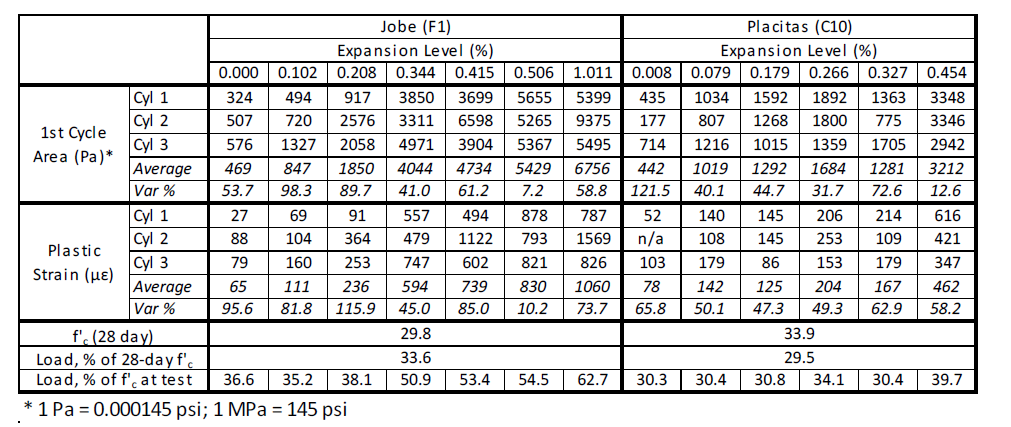
\includegraphics[width=0.8\linewidth]{Reference/GIANNINIDEF.png}
  \caption{Elastic modulus and compressive strength results for DEF cylinders[Giannini, 2012\cite{GIANNINI}]}
  \label{Giannini, 2012 DEF}
\end{figure}

\clearpage
% Bouzabata et al., (2012)

In experiments performed by Bouzabata et al.\cite{Bouzabata}, DEF expansion for restrained and stress free on mortar prisms (40x40x160 mm) were presented. The water/cement ratio was 0.55 and the sand/cement ratio was 3. The chemical composition of the Portland cement used is given in Figure \ref{Bouzabata (2012)1}. As in the previous experiments, 3.1\% of $Na_2SO_4$ was added to the mixing water. Siliceous sand known to be non-alkali-reactive was used.

\begin{figure}[h!]
  \centering
  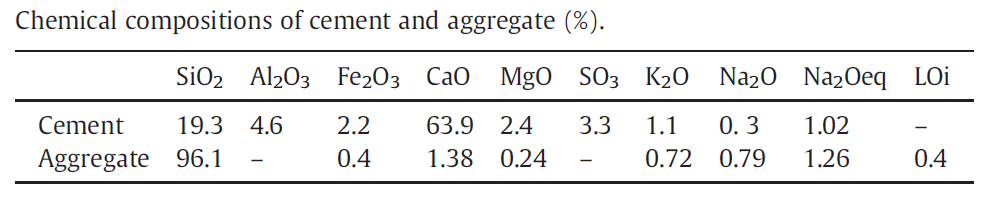
\includegraphics[width=0.8\linewidth]{Reference/Bouzabata1.png}
  \caption{Chemical compositions of cement and aggregate (\%) mortar prisms [Bouzabata et al., 2012\cite{Bouzabata}]}
  \label{Bouzabata (2012)1}
\end{figure}

After casting, some of the specimens were cured at high temperatures with the heat treatment: 1 h at 20 $^\circ$C, an increase from 20 to 80 $^\circ$C in 4 h, a constant temperature of 80 $^\circ$C for 10 h then a cooling to 20 $^\circ$C in 10 h. The specimens were steamed in metal moulds, wrapped in watertight plastic film and covered by a metal plate to prevent evaporation of water during the heat treatment. At the same time, other specimens made in the same batch were stored at 20 $^\circ$C. After cooling and demoulding, specimens were kept at 20 $^\circ$C in endogenous conditions (sealed in plastic bags) for 28 days. [Bouzabata et al., (2012)\cite{Bouzabata}]

Strains of specimens kept immersed in water after 28 days in stress-free conditions have been plotted in Figure \ref{Bouzabata (2012)2}. The specimens that had been subjected to the heat treatment during the curing period showed large expansions of between 1.3 and 2.2\% due to DEF. All the specimens in stress-free conditions exhibited mapcracking. The first significant cracks appeared for a strain of about 0.5\% (after 80 days of immersion in water). Compressive strength was measured on prismatic specimens (40x40x40 mm) at time-steps chosen according to the expansions measured on the specimens (Figure \ref{Bouzabata (2012)2}).[Bouzabata et al., (2012)\cite{Bouzabata}]

\begin{figure}[h!]
  \centering
  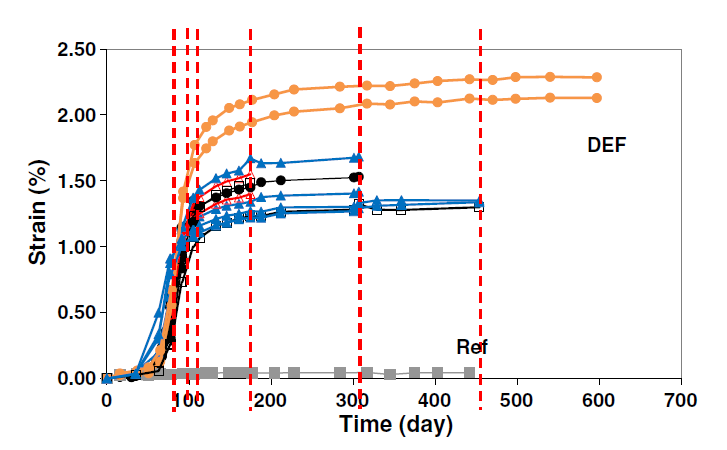
\includegraphics[width=0.8\linewidth]{Reference/Bouzabata2.png}
  \caption{Strain of specimens in stress-free conditions (each line corresponds to one specimen, specimens of a same batch are plotted with the same marker — dotted lines show the times of the mechanical tests). [Bouzabata et al., (2012)\cite{Bouzabata}]}
  \label{Bouzabata (2012)2}
\end{figure}

The evolution of the compressive strength of the reference mortar and of the mortar damaged by delayed ettringite formation have been plotted in Figure \ref{Bouzabata (2012)3}. The reference specimens showed the usual increase of compressive strength with time due to continuous cement hydration. The specimens that had been subjected to the heat treatment showed a decrease in strength around 40\%. A large strength decrease occurred mainly between 70 and 100 days, corresponding to the significant increase of expansion, and the compressive strength reached a minimum value of 25 MPa at 180 days.[Bouzabata et al., (2012)\cite{Bouzabata}]

\begin{figure}[h!]
  \centering
  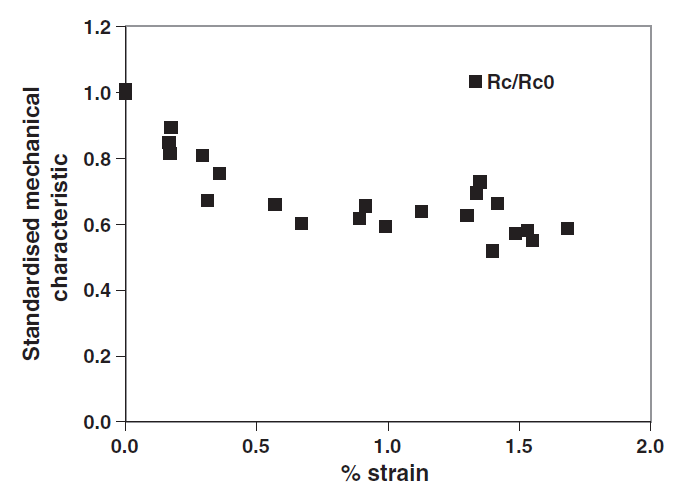
\includegraphics[width=0.8\linewidth]{Reference/Bouzabata3.png}
  \caption{Decrease of compressive strength according to DEF expansion [Bouzabata et al., 2012\cite{Bouzabata}]}
  \label{Bouzabata (2012)3}
\end{figure}


\clearpage
% M. Al Shamaa et al., 2014

Figure 2 summarizes the mix design of the concrete used in the construction of the raft foundation, done by M. Al Shamaa et al., 2014 \cite{Shamaa}. Concrete is made with calcareous
aggregates (in order to avoid the risk of alkali-aggregate reaction) and Portland cement CEM II/A-LL 42.5 R, which can be susceptible to an expansive behavior due to DEF. Concrete specimens were prepared according to the standards NF P 18-400 and NF P 18-422. Samples were cast in cylindrical molds whose dimensions are 11 cm (diameter) and 22 cm (height).

After casting, a part of concrete specimens was cured under heat treatments, shown in Figure \ref{Shamaa1}. The maximum temperature in cycle reached maximum 70$^\circ$C to expose concrete to a more severe condition by taking into account the variability of the properties of the material. Then the duration of the heat treatment was 18 days.

\begin{figure}[h!]
  \centering
  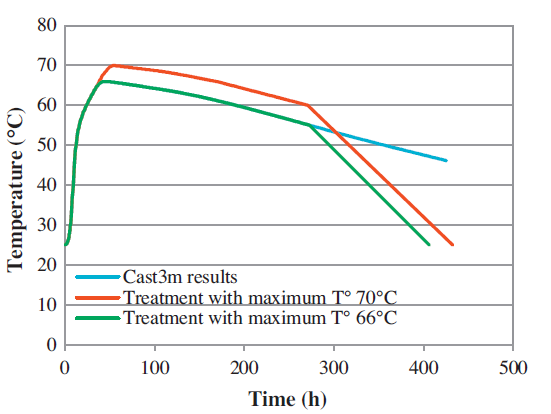
\includegraphics[width=0.8\linewidth]{Reference/Shamaa1.png}
  \caption{Experimental applied heat treatments [M. Al Shamaa et al., 2014\cite{Shamaa}]}
  \label{Shamaa1}
\end{figure}

Figure \ref{Shamaa_2} shows a comparison of compressive strength and Young’s modulus at the age of 28 days for different concretes.

\begin{figure}[h!]
  \centering
  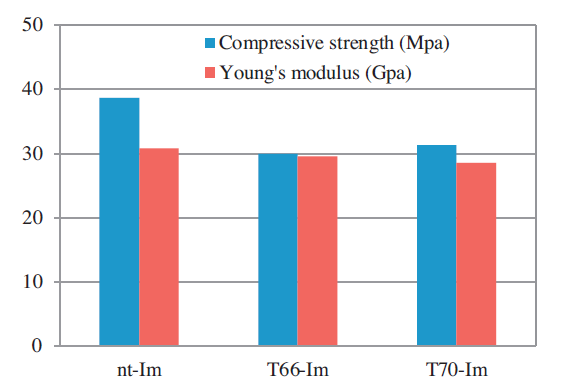
\includegraphics[width=0.8\linewidth]{Reference/Shamaa2.png}
  \caption{Effect of heat treatment on the compressive strength and Young’s modulus
at 28 days. [M. Al Shamaa et al., 2014\cite{Shamaa}]}
  \label{Shamaa_2}
\end{figure}

Due to heat treatments, a decrease appeared of approximately 20\% of the compressive strength. This decrease was observed in both concretes T70-Im and T66-Im. Thus, the application of heat curing induces a lower value of mechanical resistance before the concrete is affected by DEF.

However, the Young’s modulus does not seem to be affected by the heat treatment. On the other hand, Figure \ref{Shamaa_3} shows that the concrete T70-Im, which suffers from DEF, presents a degradation of its mechanical properties. We observe a 23\% reduction in the compressive strength when the expansion was evolved from 0.08\% at the age of 180 days to 0.20\% at the age of 390 days. This loss is also observed for the Young’s modulus and may be an indicator of the damage of the material.

\begin{figure}[h!]
  \centering
  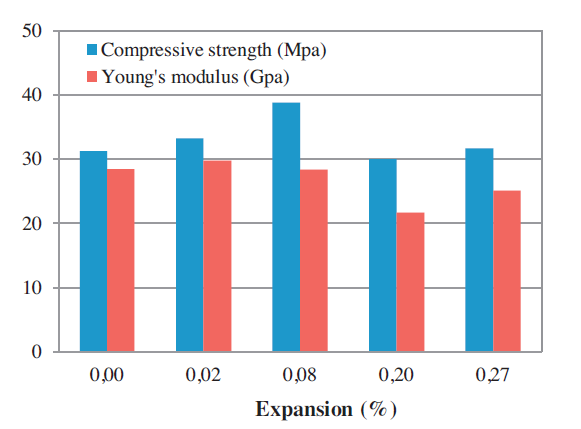
\includegraphics[width=0.8\linewidth]{Reference/Shamaa3.png}
  \caption{Relationship between the compressive strength, the Young’s modulus and
the expansion for concrete T70-Im. [M. Al Shamaa et al., 2014\cite{Shamaa}]}
  \label{Shamaa_3}
\end{figure}

However, the strength loss is not proportional to the expansion reached. In fact, we observe, according to our last measurements (at the age of 640 days when the expansion reaches 0.27\%), that the concrete tends to regain a part of its mechanical performance he had lost. This delayed re-increase is observed both on the compressive strength, the dynamic and the Young’s modulus.

These quantities have a minimum. Minima are observed at around 400 days when the inflection point of the slowdown in the expansion curve is reached Figure \ref{Shamaa_4}. On the other hand, all measurements on the concrete T66-Im concern only small expansions and the mechanical performances of this concrete was not affected until now.

\begin{figure}[h!]
  \centering
  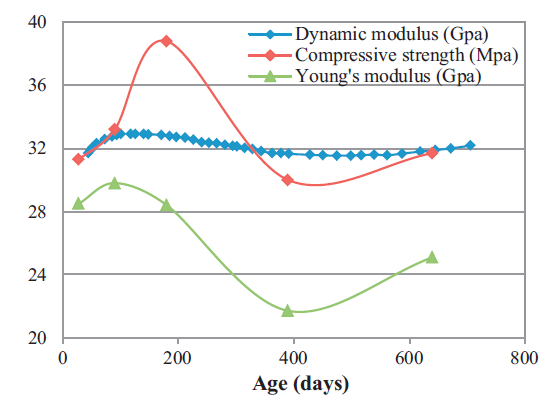
\includegraphics[width=0.8\linewidth]{Reference/Shamaa4.png}
  \caption{Mechanical properties versus time for concrete T70-Im. [M. Al Shamaa et al., 2014\cite{Shamaa}]}
  \label{Shamaa_4}
\end{figure}

\clearpage
\subsection{Summary of Experimental Result of DEF Expansion on Mechanical Properties of Concrete}

\begin{figure}[h!]
  \centering
  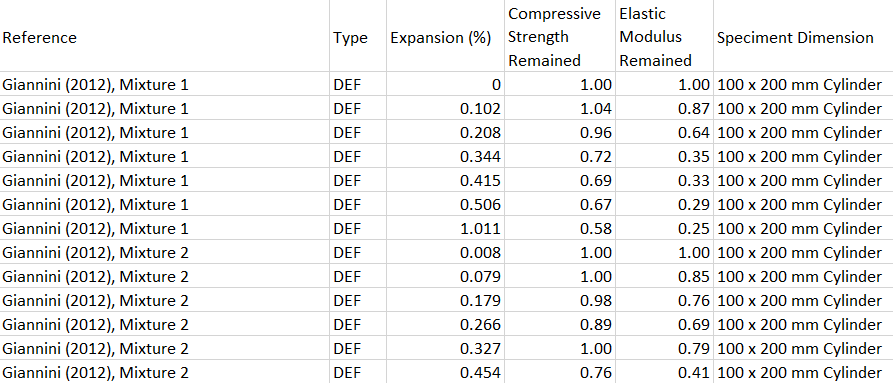
\includegraphics[width=1.0\linewidth]{Reference/GIANNINIDEFdata.png}
\end{figure}

\begin{figure}[h!]
  \centering
  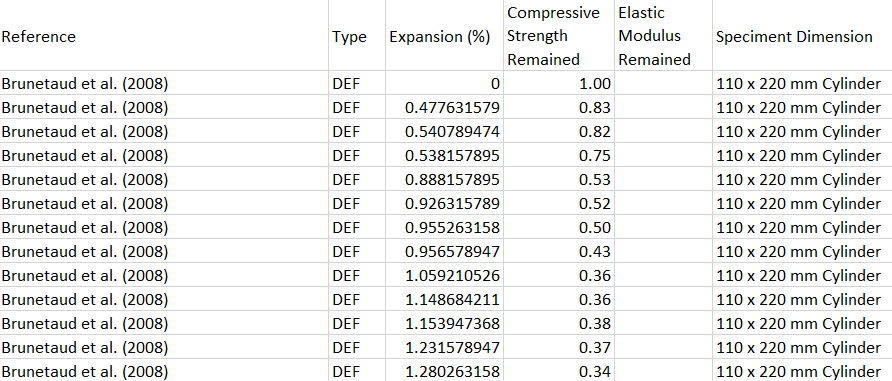
\includegraphics[width=1.0\linewidth]{Reference/BruetaudDEFdata.png}
\end{figure}

\begin{figure}[h!]
  \centering
  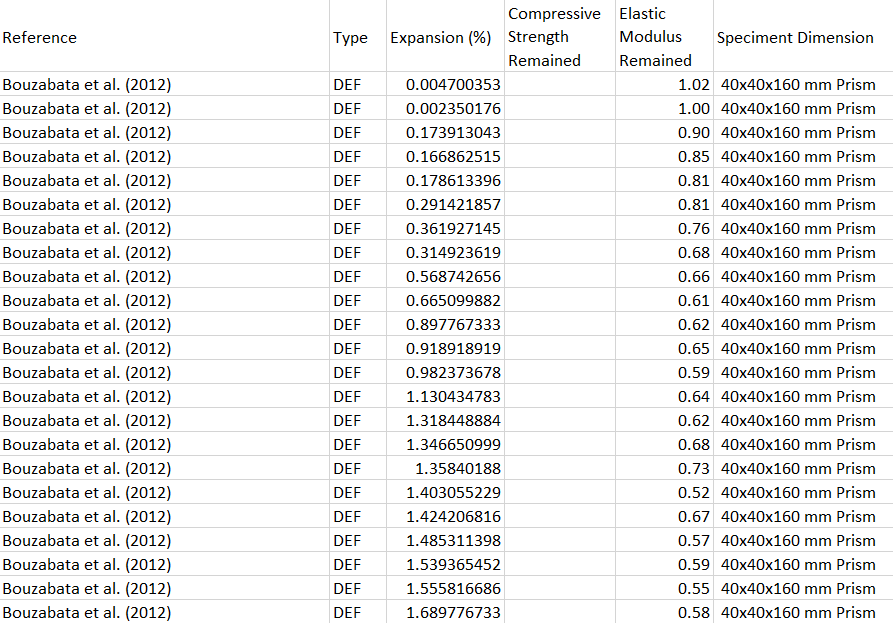
\includegraphics[width=1.0\linewidth]{Reference/BouzabataDEFdata.png}
\end{figure}

\begin{figure}[h!]
  \centering
  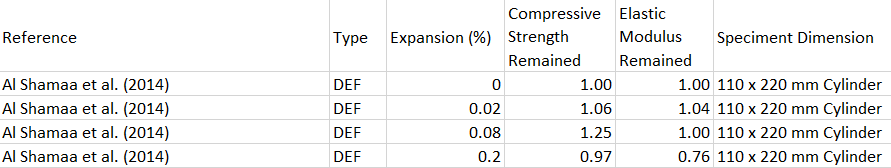
\includegraphics[width=1.0\linewidth]{Reference/ShamaaDEFdata.png}
\end{figure}
